\documentclass{ximera}

%\usepackage{todonotes}

\newcommand{\todo}{}

\usepackage{esint} % for \oiint
\ifxake%%https://math.meta.stackexchange.com/questions/9973/how-do-you-render-a-closed-surface-double-integral
\renewcommand{\oiint}{{\large\bigcirc}\kern-1.56em\iint}
\fi


\graphicspath{
  {./}
  {ximeraTutorial/}
  {basicPhilosophy/}
  {functionsOfSeveralVariables/}
  {normalVectors/}
  {lagrangeMultipliers/}
  {vectorFields/}
  {greensTheorem/}
  {shapeOfThingsToCome/}
  {dotProducts/}
  {partialDerivativesAndTheGradientVector/}
  {../productAndQuotientRules/exercises/}
  {../normalVectors/exercisesParametricPlots/}
  {../continuityOfFunctionsOfSeveralVariables/exercises/}
  {../partialDerivativesAndTheGradientVector/exercises/}
  {../directionalDerivativeAndChainRule/exercises/}
  {../commonCoordinates/exercisesCylindricalCoordinates/}
  {../commonCoordinates/exercisesSphericalCoordinates/}
  {../greensTheorem/exercisesCurlAndLineIntegrals/}
  {../greensTheorem/exercisesDivergenceAndLineIntegrals/}
  {../shapeOfThingsToCome/exercisesDivergenceTheorem/}
  {../greensTheorem/}
  {../shapeOfThingsToCome/}
  {../separableDifferentialEquations/exercises/}
  {vectorFields/}
}

\newcommand{\mooculus}{\textsf{\textbf{MOOC}\textnormal{\textsf{ULUS}}}}

\usepackage{tkz-euclide}
\usepackage{tikz}
\usepackage{tikz-cd}
\usetikzlibrary{arrows}
\tikzset{>=stealth,commutative diagrams/.cd,
  arrow style=tikz,diagrams={>=stealth}} %% cool arrow head
\tikzset{shorten <>/.style={ shorten >=#1, shorten <=#1 } } %% allows shorter vectors

\usetikzlibrary{backgrounds} %% for boxes around graphs
\usetikzlibrary{shapes,positioning}  %% Clouds and stars
\usetikzlibrary{matrix} %% for matrix
\usepgfplotslibrary{polar} %% for polar plots
\usepgfplotslibrary{fillbetween} %% to shade area between curves in TikZ
%\usetkzobj{all}
\usepackage[makeroom]{cancel} %% for strike outs
%\usepackage{mathtools} %% for pretty underbrace % Breaks Ximera
%\usepackage{multicol}
\usepackage{pgffor} %% required for integral for loops



%% http://tex.stackexchange.com/questions/66490/drawing-a-tikz-arc-specifying-the-center
%% Draws beach ball
\tikzset{pics/carc/.style args={#1:#2:#3}{code={\draw[pic actions] (#1:#3) arc(#1:#2:#3);}}}



\usepackage{array}
\setlength{\extrarowheight}{+.1cm}
\newdimen\digitwidth
\settowidth\digitwidth{9}
\def\divrule#1#2{
\noalign{\moveright#1\digitwidth
\vbox{\hrule width#2\digitwidth}}}




% \newcommand{\RR}{\mathbb R}
% \newcommand{\R}{\mathbb R}
% \newcommand{\N}{\mathbb N}
% \newcommand{\Z}{\mathbb Z}

\newcommand{\sagemath}{\textsf{SageMath}}


%\renewcommand{\d}{\,d\!}
%\renewcommand{\d}{\mathop{}\!d}
%\newcommand{\dd}[2][]{\frac{\d #1}{\d #2}}
%\newcommand{\pp}[2][]{\frac{\partial #1}{\partial #2}}
% \renewcommand{\l}{\ell}
%\newcommand{\ddx}{\frac{d}{\d x}}

% \newcommand{\zeroOverZero}{\ensuremath{\boldsymbol{\tfrac{0}{0}}}}
%\newcommand{\inftyOverInfty}{\ensuremath{\boldsymbol{\tfrac{\infty}{\infty}}}}
%\newcommand{\zeroOverInfty}{\ensuremath{\boldsymbol{\tfrac{0}{\infty}}}}
%\newcommand{\zeroTimesInfty}{\ensuremath{\small\boldsymbol{0\cdot \infty}}}
%\newcommand{\inftyMinusInfty}{\ensuremath{\small\boldsymbol{\infty - \infty}}}
%\newcommand{\oneToInfty}{\ensuremath{\boldsymbol{1^\infty}}}
%\newcommand{\zeroToZero}{\ensuremath{\boldsymbol{0^0}}}
%\newcommand{\inftyToZero}{\ensuremath{\boldsymbol{\infty^0}}}



% \newcommand{\numOverZero}{\ensuremath{\boldsymbol{\tfrac{\#}{0}}}}
% \newcommand{\dfn}{\textbf}
% \newcommand{\unit}{\,\mathrm}
% \newcommand{\unit}{\mathop{}\!\mathrm}
% \newcommand{\eval}[1]{\bigg[ #1 \bigg]}
% \newcommand{\seq}[1]{\left( #1 \right)}
% \renewcommand{\epsilon}{\varepsilon}
% \renewcommand{\phi}{\varphi}


% \renewcommand{\iff}{\Leftrightarrow}

% \DeclareMathOperator{\arccot}{arccot}
% \DeclareMathOperator{\arcsec}{arcsec}
% \DeclareMathOperator{\arccsc}{arccsc}
% \DeclareMathOperator{\si}{Si}
% \DeclareMathOperator{\scal}{scal}
% \DeclareMathOperator{\sign}{sign}


%% \newcommand{\tightoverset}[2]{% for arrow vec
%%   \mathop{#2}\limits^{\vbox to -.5ex{\kern-0.75ex\hbox{$#1$}\vss}}}
% \newcommand{\arrowvec}[1]{{\overset{\rightharpoonup}{#1}}}
% \renewcommand{\vec}[1]{\arrowvec{\mathbf{#1}}}
% \renewcommand{\vec}[1]{{\overset{\boldsymbol{\rightharpoonup}}{\mathbf{#1}}}}

% \newcommand{\point}[1]{\left(#1\right)} %this allows \vector{ to be changed to \vector{ with a quick find and replace
% \newcommand{\pt}[1]{\mathbf{#1}} %this allows \vec{ to be changed to \vec{ with a quick find and replace
% \newcommand{\Lim}[2]{\lim_{\point{#1} \to \point{#2}}} %Bart, I changed this to point since I want to use it.  It runs through both of the exercise and exerciseE files in limits section, which is why it was in each document to start with.

% \DeclareMathOperator{\proj}{\mathbf{proj}}
% \newcommand{\veci}{{\boldsymbol{\hat{\imath}}}}
% \newcommand{\vecj}{{\boldsymbol{\hat{\jmath}}}}
% \newcommand{\veck}{{\boldsymbol{\hat{k}}}}
% \newcommand{\vecl}{\vec{\boldsymbol{\l}}}
% \newcommand{\uvec}[1]{\mathbf{\hat{#1}}}
% \newcommand{\utan}{\mathbf{\hat{t}}}
% \newcommand{\unormal}{\mathbf{\hat{n}}}
% \newcommand{\ubinormal}{\mathbf{\hat{b}}}

% \newcommand{\dotp}{\bullet}
% \newcommand{\cross}{\boldsymbol\times}
% \newcommand{\grad}{\boldsymbol\nabla}
% \newcommand{\divergence}{\grad\dotp}
% \newcommand{\curl}{\grad\cross}
%\DeclareMathOperator{\divergence}{divergence}
%\DeclareMathOperator{\curl}[1]{\grad\cross #1}
% \newcommand{\lto}{\mathop{\longrightarrow\,}\limits}

% \renewcommand{\bar}{\overline}

\colorlet{textColor}{black}
\colorlet{background}{white}
\colorlet{penColor}{blue!50!black} % Color of a curve in a plot
\colorlet{penColor2}{red!50!black}% Color of a curve in a plot
\colorlet{penColor3}{red!50!blue} % Color of a curve in a plot
\colorlet{penColor4}{green!50!black} % Color of a curve in a plot
\colorlet{penColor5}{orange!80!black} % Color of a curve in a plot
\colorlet{penColor6}{yellow!70!black} % Color of a curve in a plot
\colorlet{fill1}{penColor!20} % Color of fill in a plot
\colorlet{fill2}{penColor2!20} % Color of fill in a plot
\colorlet{fillp}{fill1} % Color of positive area
\colorlet{filln}{penColor2!20} % Color of negative area
\colorlet{fill3}{penColor3!20} % Fill
\colorlet{fill4}{penColor4!20} % Fill
\colorlet{fill5}{penColor5!20} % Fill
\colorlet{gridColor}{gray!50} % Color of grid in a plot

\newcommand{\surfaceColor}{violet}
\newcommand{\surfaceColorTwo}{redyellow}
\newcommand{\sliceColor}{greenyellow}




\pgfmathdeclarefunction{gauss}{2}{% gives gaussian
  \pgfmathparse{1/(#2*sqrt(2*pi))*exp(-((x-#1)^2)/(2*#2^2))}%
}


%%%%%%%%%%%%%
%% Vectors
%%%%%%%%%%%%%

%% Simple horiz vectors
\renewcommand{\vector}[1]{\left\langle #1\right\rangle}


%% %% Complex Horiz Vectors with angle brackets
%% \makeatletter
%% \renewcommand{\vector}[2][ , ]{\left\langle%
%%   \def\nextitem{\def\nextitem{#1}}%
%%   \@for \el:=#2\do{\nextitem\el}\right\rangle%
%% }
%% \makeatother

%% %% Vertical Vectors
%% \def\vector#1{\begin{bmatrix}\vecListA#1,,\end{bmatrix}}
%% \def\vecListA#1,{\if,#1,\else #1\cr \expandafter \vecListA \fi}

%%%%%%%%%%%%%
%% End of vectors
%%%%%%%%%%%%%

%\newcommand{\fullwidth}{}
%\newcommand{\normalwidth}{}



%% makes a snazzy t-chart for evaluating functions
%\newenvironment{tchart}{\rowcolors{2}{}{background!90!textColor}\array}{\endarray}

%%This is to help with formatting on future title pages.
\newenvironment{sectionOutcomes}{}{}



%% Flowchart stuff
%\tikzstyle{startstop} = [rectangle, rounded corners, minimum width=3cm, minimum height=1cm,text centered, draw=black]
%\tikzstyle{question} = [rectangle, minimum width=3cm, minimum height=1cm, text centered, draw=black]
%\tikzstyle{decision} = [trapezium, trapezium left angle=70, trapezium right angle=110, minimum width=3cm, minimum height=1cm, text centered, draw=black]
%\tikzstyle{question} = [rectangle, rounded corners, minimum width=3cm, minimum height=1cm,text centered, draw=black]
%\tikzstyle{process} = [rectangle, minimum width=3cm, minimum height=1cm, text centered, draw=black]
%\tikzstyle{decision} = [trapezium, trapezium left angle=70, trapezium right angle=110, minimum width=3cm, minimum height=1cm, text centered, draw=black]


\title{Lines}

\begin{document}

\begin{abstract}
slope
\end{abstract}
\maketitle



Linear functions exhibit a constant growth rate or constant rate of change and this is represented graphically by the slope of the function's graph, which is a line.


\begin{definition} \textbf{\textcolor{green!50!black}{Slope}} \\


\textbf{Slope} is a measurement of the tilt of a line.


\[
slope = \frac{rise}{run} = \frac{\Delta vertical}{\Delta horizontal}
\]


If $(x_1, y_1)$ and $(x_2, y_2)$ are two points on a line, then the slope can be calculated as

\[
slope = \frac{rise}{run} = \frac{\Delta vertical}{\Delta horizontal} = \frac{y_2 - y_1}{x_2 - x_1}
\]



\end{definition}


$m$ is a common symbol for slope in linear equations.




\begin{observation}

$\blacktriangleright$ Slope tells us how a line is tilted.


\begin{itemize}
\item If the slope is positive, then the line slants \wordChoice{\choice[correct]{uphill} \choice{downhill}}  to the right.
\item If the slope is negative, then the line slants \wordChoice{\choice{uphill} \choice[correct]{downhill}}  to the right.
\item If the slope is zero, then the line is horizontal.
\end{itemize}


\begin{itemize}
\item Steeper lines have \wordChoice{\choice{smaller} \choice[correct]{larger}} slopes.
\item Flatter lines have \wordChoice{\choice[correct]{smaller} \choice{larger}} slopes.
\end{itemize}

\end{observation}



Suppose we have a line that contains the point $(a,b)$ and slope $m$.  Let $(x,y)$ represent any other point on the line.  Then,



\[
\frac{y-b}{x-a} = m
\]

This can be rewritten as $y - b = m(x - a)$. We call this the \textbf{\textcolor{purple!85!blue}{point-slope}} form of a line.  This equaiton can be rewritten as $y = m(x - a) + b$, which can be viewed as a formula for a function: $y(x) = m(x - a) + b$ \\




\begin{itemize}
\item lines are curves (collections of dots) that exhibit a constant slope.
\item linear equations are satisfied by the coordinates of each dot on a line.
\item linear functions are functions with a constant rate of change.
\item slope is the graphical representation of rate of change.
\end{itemize}
















Let $f(x)$ be a linear function.  Then, $f(x)$ has a formula of the form $f(x) = m(x-a) + f(a)$.  $m$ is called the rate-of-change of $f(x)$.


Suppose we have the Cartesian plane displaying the graph of $f(x)$ with the vertical axis, $y$, representing $f(x)$.  Then we have $y = f(x)$, which gives us $y = m(x-a) + f(a)$, which is a linear equation, which is the equation for the plotted curve - a line in this case.

\begin{itemize}
\item We have an algebraic object - the equation, which describes the pairs or points. 
\item We have a geometric object - the line, which is a collection of points. 
\item We have an algebraic object - the function $f(x)$, which collects all of the pieces into a single package. 
\end{itemize}


This algebraic - geometric connection connects many algebraic characteristics with graphical features.

















\subsection*{Parallel}

\textbf{Parallel lines} are lines with the same slope.  They are graphs of linear functions with the same rate of change.


Let $f(x) = \frac{1}{2} x - 4$ and $g(x) = \frac{1}{2} x + 1$.




Below are the graphs of $y = f(x)$ and $y = g(x)$.


\begin{image}
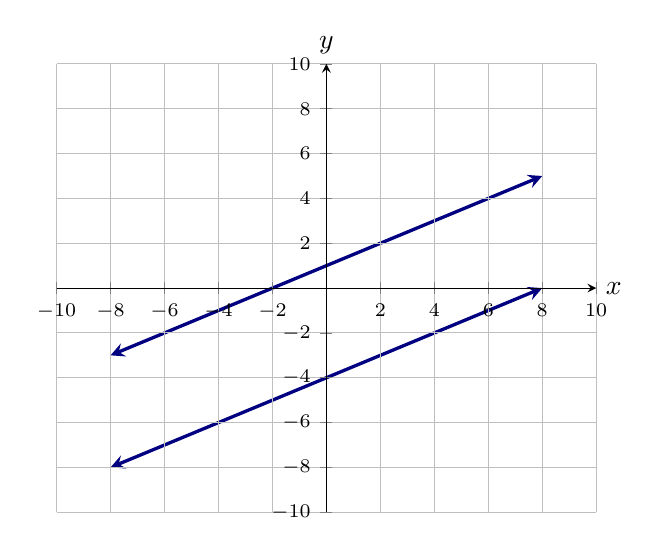
\begin{tikzpicture}
     \begin{axis}[
            	domain=-10:10, ymax=10, xmax=10, ymin=-10, xmin=-10,
            	axis lines =center, xlabel=$x$, ylabel=$y$, grid = major,
                ytick={-10,-8,-6,-4,-2,2,4,6,8,10},
                xtick={-10,-8,-6,-4,-2,2,4,6,8,10},
                ticklabel style={font=\scriptsize},
            	every axis y label/.style={at=(current axis.above origin),anchor=south},
            	every axis x label/.style={at=(current axis.right of origin),anchor=west},
            	axis on top,
          		]

        
        \addplot [draw=penColor, very thick, smooth, domain=(-8:8),<->] {0.5*x+1};
        \addplot [draw=penColor, very thick, smooth, domain=(-8:8),<->] {0.5*x-4};




    \end{axis}
\end{tikzpicture}
\end{image}



If two linear functions have the same rate of change, then they must differ by only a constant. 


In the example above, $f(x) - g(x) = -5$ or $f(x) = g(x) - 5$. \\

Graphically, this means that either line can be shifted vertically by $5$ units to land on the other.










\subsection*{Perpendicular}

\textbf{Prependicular lines} are lines that form a right angle.   


Below are the graphs of two lines, $L_1$ and $L_2$, whch intersect at the point $(a,b)$.


\begin{image}
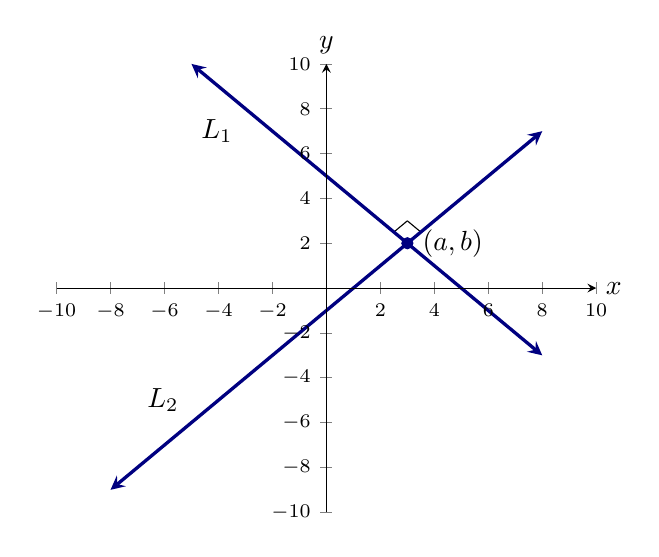
\begin{tikzpicture}
     \begin{axis}[
            	domain=-10:10, ymax=10, xmax=10, ymin=-10, xmin=-10,
            	axis lines =center, xlabel=$x$, ylabel=$y$, 
                ytick={-10,-8,-6,-4,-2,2,4,6,8,10},
                xtick={-10,-8,-6,-4,-2,2,4,6,8,10},
                ticklabel style={font=\scriptsize},
            	every axis y label/.style={at=(current axis.above origin),anchor=south},
            	every axis x label/.style={at=(current axis.right of origin),anchor=west},
            	axis on top,
          		]

        

        \addplot [draw=black, thin, smooth, domain=(3:3.5)] {-x+6};
        \addplot [draw=black, thin, smooth, domain=(2.5:3)] {x};

        \addplot [draw=penColor, very thick, smooth, domain=(-8:8),<->] {x-1};
        \addplot [draw=penColor, very thick, smooth, domain=(-5:8),<->] {-x+5};
        \addplot[color=penColor,fill=penColor,only marks,mark=*] coordinates{(3,2)};
        \node at (axis cs:3.2,2) [anchor=west] {$(a, b)$};

        \node at (axis cs:-5,7) [anchor=west] {$L_1$};
        \node at (axis cs:-7,-5) [anchor=west] {$L_2$};




    \end{axis}
\end{tikzpicture}
\end{image}



The equation of line $L_1$ would be $y = m(x-a) + b$ and $L_2$ would have the equation $y = n(x-a) + b$, where $m$ and $n$ are their respective slopes.



\begin{question}
Each line above contains the point $(a, b)$. Let's select another point on each line.

Each line has a point where $x = a + 1$.


$\blacktriangleright$  For $L_1$, the corresponding y-coordinate would be $y = \answer{m+b}$ \\

$\blacktriangleright$  For $L_2$, the corresponding y-coordinate would be $y = \answer{n+b}$

\end{question}




\begin{image}
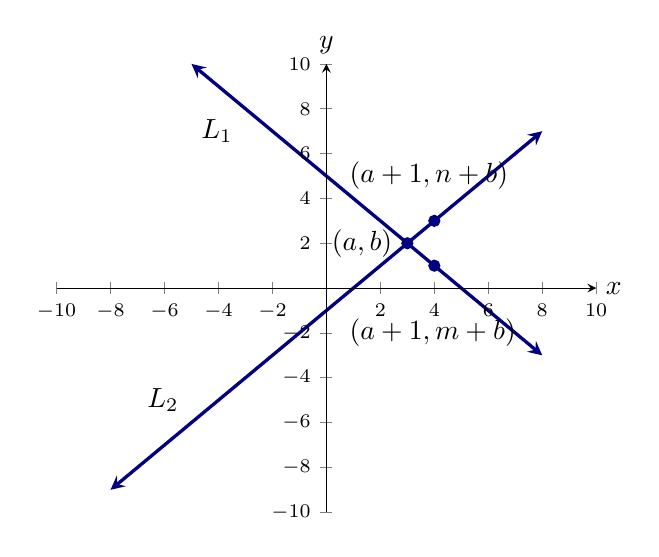
\begin{tikzpicture}
     \begin{axis}[
            	domain=-10:10, ymax=10, xmax=10, ymin=-10, xmin=-10,
            	axis lines =center, xlabel=$x$, ylabel=$y$, 
                ytick={-10,-8,-6,-4,-2,2,4,6,8,10},
                xtick={-10,-8,-6,-4,-2,2,4,6,8,10},
                ticklabel style={font=\scriptsize},
            	every axis y label/.style={at=(current axis.above origin),anchor=south},
            	every axis x label/.style={at=(current axis.right of origin),anchor=west},
            	axis on top,
          		]

        
        \addplot [draw=penColor, very thick, smooth, domain=(-8:8),<->] {x-1};
        \addplot [draw=penColor, very thick, smooth, domain=(-5:8),<->] {-x+5};
        \addplot[color=penColor,fill=penColor,only marks,mark=*] coordinates{(3,2)};
        \node at (axis cs:2.8,2) [anchor=east] {$(a, b)$};

        \addplot[color=penColor,fill=penColor,only marks,mark=*] coordinates{(4,3)};
        \node at (axis cs:0.5,5) [anchor=west] {$(a+1, n+b)$};

        \addplot[color=penColor,fill=penColor,only marks,mark=*] coordinates{(4,1)};
        \node at (axis cs:0.5,-2) [anchor=west] {$(a+1, m+b)$};

        \node at (axis cs:-5,7) [anchor=west] {$L_1$};
        \node at (axis cs:-7,-5) [anchor=west] {$L_2$};




    \end{axis}
\end{tikzpicture}
\end{image}


Since we have a right angle, these points are corners of a right triangle.  Therefore, the lengths have to satisfy the Pythagorean Theorem.  



\begin{question}

The lengths are

\begin{itemize}
\item lower side : $\sqrt{(a + 1 - a)^2 + (n + b) - b)^2} = \sqrt{\answer{1 + n^2}}$
\item higher side : $\sqrt{(a + 1 - a)^2 + (m + b) - b)^2} = \sqrt{\answer{1 + m^2}}$
\item hypotenuse : $\answer{m-n}$
\end{itemize}

\end{question}





The Pythagorean Theorem gives us


\begin{align*}
\left(\sqrt{1 + n^2}\right)^2 + \left(\sqrt{1 + m^2}\right)^2 & = (m-n))^2 \\
1 + n^2 + 1 + m^2 & = m^2 - 2 m n + n^2  \\
2 & = -2 m n \\
1 & = -m n \\
\frac{1}{-m} & = n
\end{align*}

The slopes are negative reciprocals of each other. \\


\begin{itemize}
\item The slopes of perpendicular lines are negative reciprocals.
\item The product of the slopes of perpendicular lines equals $-1$.
\end{itemize}



















\subsection*{Intercepts}


Almost every line intersects both the horizontal and vertical axes.  These points are called the \textbf{intercepts} of the line.  Horizontal and vertical lines have one intercept, unless they just happen to be one of the axes. \\

If we think of the line as the graph of a linear function, $f$, then the horizontal intercept looks like $(a, 0)$, which means $f(a)=0$ and $a$ is the zero of $f$. In this case, our formula looks like $f(x) = m (x-a)$ and $(x - a)$ is a factor of the formula.



The trio 

\begin{itemize}
\item \textbf{\textcolor{blue!55!black}{horizontal intercepts}} 
\item \textbf{\textcolor{blue!55!black}{factors}} 
\item \textbf{\textcolor{blue!55!black}{zeros}} 
\end{itemize}

all represent the same idea. \\



The vertical intercept looks like $(0, b)$, where $f(x) = m(x-0)+b = m \, x + b$.  This is not as valuable as the horizontal intercept, which corresponds to a zero and a factor. \\










\subsection*{Horizontal Lines} 

Horizontal lines have equations of the form $y = y_0$, where the $y$ is the name of the vertical axis. You can view this equation as $y = 0 \cdot x + y_0$ to see that every point on this line is of the form $(x, y_0)$, making it horizontal.





\begin{example} Horizontal Line





The equation of this line is $w=3$.  

\begin{image}
\begin{tikzpicture}
     \begin{axis}[
            	domain=-10:10, ymax=10, xmax=10, ymin=-10, xmin=-10,
            	axis lines =center, xlabel=$t$, ylabel=$w$,
                ytick={-10,-8,-6,-4,-2,2,4,6,8,10},
                xtick={-10,-8,-6,-4,-2,2,4,6,8,10},
                ticklabel style={font=\scriptsize},
            	every axis y label/.style={at=(current axis.above origin),anchor=south},
            	every axis x label/.style={at=(current axis.right of origin),anchor=west},
            	axis on top,
          		]

        
        \addplot [draw=penColor, very thick, smooth, domain=(-8:8),<->] {3};






    \end{axis}
\end{tikzpicture}
\end{image}

Every point on this line is of the form $\left(t_0, \answer{3}\right)$. It is the graph of the constant function $f(t)=3$.


\end{example}
Horizontal lines are graphs of constant functions.  Constant functions are linear functions with a growth rate of $0$. \\
















\subsection*{Vertical Lines} 


Vertical lines have equations of the form $x = x_0$, where the $x$ is the name of the horizontal axis. You can view this equation as $x = 0 \cdot y + x_0$ to see that every point on this line is of the form $(x_0,y)$, making it vertical.





\begin{example} Vertical Line


The equation of this line is $h=4$. 

\begin{image}
\begin{tikzpicture}
     \begin{axis}[
            	domain=-10:10, ymax=10, xmax=10, ymin=-10, xmin=-10,
            	axis lines =center, xlabel=$h$, ylabel=$g$, 
                ytick={-10,-8,-6,-4,-2,2,4,6,8,10},
                xtick={-10,-8,-6,-4,-2,2,4,6,8,10},
                ticklabel style={font=\scriptsize},
            	every axis y label/.style={at=(current axis.above origin),anchor=south},
            	every axis x label/.style={at=(current axis.right of origin),anchor=west},
            	axis on top,
          		]

        
        \addplot [draw=penColor, very thick, smooth, domain=(-8:8),<->] ({4},{x});






    \end{axis}
\end{tikzpicture}
\end{image}

Every point on this line is of the form $\left(\answer{4}, g_0\right)$. This graph corresponds to no linear function, because the single domain number $4$ is paired with more than one codomain number.


\end{example}

Every line is the graph of a linear function, except vertical lines. \\






























\subsection*{Product Form}


We have many forms for writing linear equations and formulas for linear functions.



$\blacktriangleright$ Point-Slope Form

Given a point on a line, $(a, f(a))$, and the slope, $m$, we can write the formula as $f(x) = m(x-a) + f(a)$. This emphasizes the behavior around $a$.



$\blacktriangleright$ Slope-Intercept Form

If we choose our point to be the vertical intercept $(0, b)$, then the slope-intercept form looks like $f(x) = m \, x + f(0)$ or $f(x) = m \, x + b$.



These are both sums.


However, our interest focuses on zeros of the function, which we would like to correspond to factors in our formulas.  




\begin{model}



As long as $m \ne 0$, we can take our sum and transform it into a product.




\begin{align*}
f(x) & = m(x-a) + f(a) \\
& = m \left(x - a + \frac{f(a)}{\answer{m}}\right)  \\
& = m \left(x - \left(a - \frac{f(a)}{m}\right)\right) 
\end{align*}



Since $f$ is linear, $f$ has one zero.  It is $a - \frac{f(a)}{m}$.  It is visually encoded as the horizontal intercept, $\left(a - \frac{f(a)}{m}, 0\right)$.


This zero will always exist as long as $m \ne 0$.


\end{model}



\begin{example}  Factored Form



Let $K(t) = 3t - 15$.


$5$ is the only root of $K$.  We can rewrite this formula in factored form knowing that $t-5$ has to be a factor.


$K(t) = 3 \left(t - \answer{5} \right)$.



Since $5$ is the only root of $K(t)$, we know that $\left(\answer{5}, \answer{0}\right)$ is the only $t$-intercept of the corresponding line.  \\

In either form, the coefficient of $t$ is $\answer{3}$.  \\

This coefficent measures the rate of change of $K$ and the slope of the line.

\end{example}




















\begin{center}
\textbf{\textcolor{green!50!black}{ooooo-=-=-=-ooOoo-=-=-=-ooooo}} \\

more examples can be found by following this link\\ \link[More Examples of Linear Functions]{https://ximera.osu.edu/csccmathematics/precalculus1/precalculus1/linearFunctions/examples/exampleList}

\end{center}












\end{document}

